\documentclass[12pt]{article}
\usepackage[utf8]{inputenc}
\usepackage[T1]{fontenc}
\usepackage[french]{babel}
\usepackage{graphicx}
\usepackage[top=3cm,bottom=2.5cm,left=2cm,right=2cm]{geometry}

\renewcommand{\contentsname}{Sommaire}
\renewcommand{\thesection}{\Roman{section} - }
\renewcommand{\thesubsection}{\Alph{subsection}) }


\title{License SPI -- Projet Auralisation}
\author{Thomas \textsc{Lechat} \and Xin \textsc{Wang} \and Mathieu \textsc{Gaborit}}
\date{Note de synthèse 2 -- Novembre 2012}
\begin{document} \maketitle

\tableofcontents
\newpage

\section{Discussion autour des approximations} % {{{

Depuis le début du projet, le procédé de mesure de réponse impulsionnelle a été examiné presque sous tous ses angles.

En fait, une partie des problèmes intrinsèques à celui-ci n'avaient pas été pris en compte, il sont donc détaillés dans
les paragraphes qui suivent.

\paragraph{Source omnidirectionnelle}

La mesure de la réponse impulsionnelle est assujettie à l'utilisation d'une source la moins directive possible.
En effet, on cherche à caractériser la salle à partir de la mesure d'un son direct et de ses réflexions, il ne faut donc
pas qu'une direction soit privilégiée par la directivité de la source.

Ce problème est particulièrement gènant en hautes fréquences, pour lesquelles la directivité de la source augmente
sensiblement.

Dans la recherche d'une source intéressante, le ballon de baudruche avait jusqu'alors été retenu.
Seulement, compte tenu de l'éclatement du ballon, celui-ci n'est pas réellement omni-directionnel (il est directif,
principalement vers le point où il est percé).

Ce n'est pas forcément très grave, mais des mesures avec une source un peu plus omni-directionnelle pourraient être
intéressantes, à titre de comparaison du moins.

\paragraph{Impulsion infiniment courte}

Il s'agit de mesurer une réponse impulsionnelle (RI), soit, la réponse d'une salle donnée à une impulsion.

Une impulsion est, par définition d'amplitude très grande devant le bruit de fond et de durée infiniment courte
(idéalement, un Dirac). Même si mathématiquement cette définition ne pose aucun problème, physiquement, elle est
fausse.

En effet, le temps de réponse d'un haut-parleur est fini et, selon le temps de réverbération de la salle, pourrait ne
pas être complètement négligeable. Il en va de même pour le ballon qui, même s'il éclate vite, n'éclate pas
instantanément.

Finalement, on ne mesure pas la réponse de la salle à une impulsion mais la réponse de la salle à presque une impulsion,
on obtient donc presque une RI.

\paragraph{Réponse en fréquence parfaite}

Enfin, il a été admis que la bande passante des sources était infinie et plate.

Un signal présentant ces caractéristiques serait... un dirac. Or, d'après le point précédent, il n'est pas aisé de
générer un tel signal.
\paragraph{Comparaison entre convolution physique et mathématique}

Il a été proposé de comparer la mesure d'un signal émis dans la salle et d'un signal convolué avec la RI de cette salle.

Cela pose un problème du même acabit que les précédents : si le signal sort de la bande passante de la chaine
d'excitation (particulièrement de celle du haut-parleur) alors celui-ci est modifié parce cette chaine (qui n'est pas du
tout parfaite).

Il faudrait donc comparer le signal émis dans la pièce réellement et le signal "découpé" par la bande-passante du
haut-parleur convolué avec la RI de la salle.

Un moyen simple de règler le problème serait de procéder comme suit :

\begin{enumerate}
    \item monter une chaine d'excitation et de mesure en chambre anéchoïque;
    \item mesurer le signal voulu émis par cette chaine;
    \item diviser le signal obtenu par la réponse en fréquences de la chaine de mesure (on obtient un signal A);
    \item convoluer ce signal avec la RI de la salle (on obtient un signal B);
    \item déplacer la chaine d'excitation dans la salle cible;
    \item émettre le signal A avec la même chaine d'excitation et le mesurer (on obtient un signal C);
    \item diviser le signal C par la réponse en fréquence de la chaine de mesure (on obtient un signal D);
    \item comparer D et B.
\end{enumerate}

Il s'agit alors d'une comparaison correcte entre un même signal émis directement dans la salle d'une part et convolué
avec la RI de cette salle de l'autre.

Ces quatre approximations sont gènantes mais mineures, en effet, même si elles rendent imparfait le procédé, elles
n'empècheront pas de continuer le projet. Il faudra simplement, au moment de tirer des conclusions, rester conscient de
ces imprécisions.


Il faut toutefois leur ajouter les deux points suivants :

\begin{itemize}
    \item la mesure n'est pas celle de la RI de la salle mais celle de la salle et de ce qui s'y trouve, pour une position de la
        source et du/des capteur(s) donnée(s);
    \item la bande-passante et les arondis de quantification (au moment de l'acquisition) viennent s'ajouter aux
        imprécisions, le matériel n'est pas transparent pour le signal;
\end{itemize}

Finalement, il s'agit d'être conscient que des compromis sont faits pour les mesures. Ceux-ci pourraient conduire à de
petits défauts d'interprétation.

% }}}
\section{Compte Rendu séance 2} % {{{

Le montage est présenté en figure~\ref{salle}.

\begin{figure}[h]
    \vfill\begin{center}
        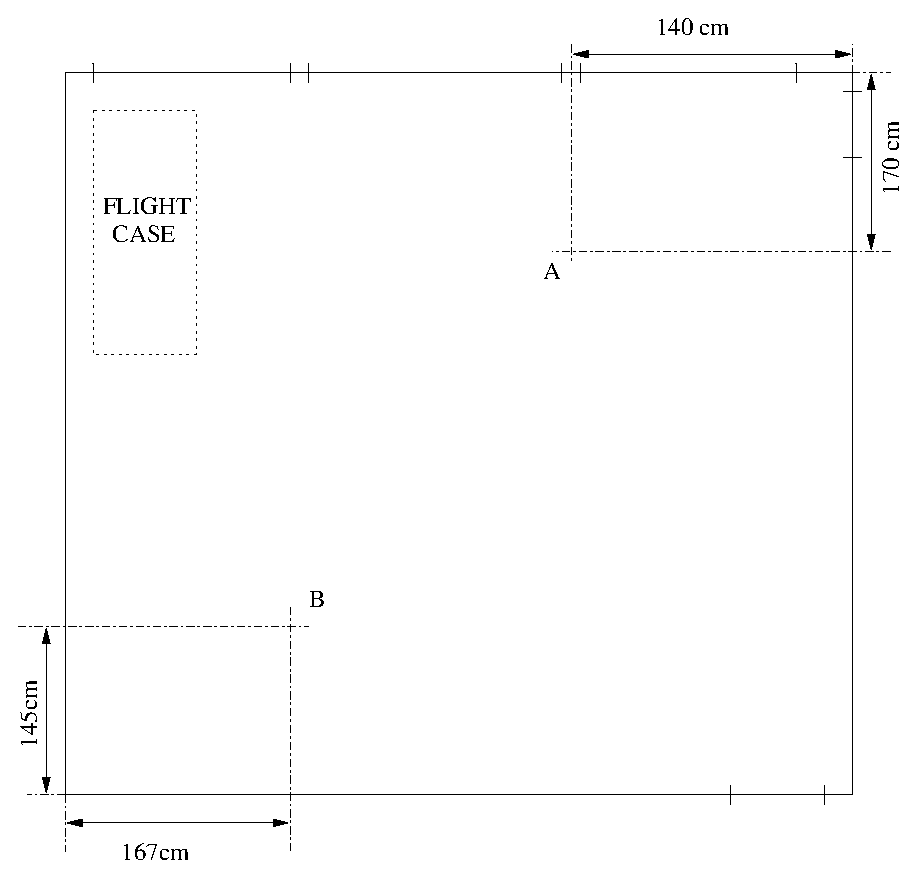
\includegraphics[scale=0.75]{schema_salle.eps}
    \end{center}\vfill
    \caption{\label{salle} Schéma de la salle de mesure. La source est en B, les capteurs (tête et micro) sont tour à
tour placés en A. Les 3 ouvertures présentes dans le mur derrière les capteurs sont des vitres.}
\end{figure}

Au cours de la séance, il s'est agit de mesurer la réponse impulsionnelle de la salle.

\paragraph{Problèmes d'acquisition}
L'acquisition a, dans un premier temps posé problème.
Après avoir changé de cable, de carte d'acquisition et de micro, c'est finalement un n-ième changement de câble qui a
résolu le problème. Merci à MM. Lihoreau et Dalmont pour leur aide.

\paragraph{Fabrication de câble}
Afin de relier le pré-amplificateur de la tête artificielle à la carte d'acquisition. Il s'agit d'un cable Jack 6.35
Stéréo $\rightarrow$ Double banane (masse distribuée).

Les mesures sont faites avec une carte d'acquisition NI-9234 (pour pouvoir couper l'alimentation ICP en cas de mesures à
la tête artificielle).

Trois prises de réponses impulsionnelles sont mesurées :

\begin{itemize}
    \item deux avec un micro (RI monaurale)
    \item une avec la tête (RI binaurale)
\end{itemize}

Les spectres de ces réponses sont donnés en figures~\ref{spectre1} et~\ref{spectre2}.
Il faut noter qu'avant le tracé des spectres, la valeur moyenne du signal lui est retranchée (pour éviter de "tasser" le
spectre avec un offset trop important).

\begin{figure}[h]
    \vfill\begin{center}
        \includegraphics[scale=0.6]{ris_monaurales.png}
    \end{center}\vfill
    \caption{\label{spectre1} Réponses fréquentielles correspondant aux réponses impulsionnelles monaurales mesurées}
\end{figure}

\begin{figure}[h]
    \vfill\begin{center}
        \includegraphics[scale=0.6]{ri_binaurale.png}
    \end{center}\vfill
    \caption{\label{spectre2} Réponses fréquentielles correspondant à la réponse impulsionnelle binaurale mesurée. Les
    cannaux droit et gauche sont séparés.}
\end{figure}

% }}}
\section{Travail de la prochaine séance} % {{{

Au cours de la prochaine séance, il faudra particulièrement mettre l'accent sur la convolution d'un signal anéchoïque
avec les 3 RI mesurées. Ensuite, il s'agira de reconstituer des fichiers WAV et d'écouter et commenter le rendu.

Pendant ce temps, il pourrait être bon de mesurer un signal anéchoïque (transmis par une chaine d'excitation limitée) en
salle anéchoïque et d'essayer de le convoluer aussi avec les RI pour comparaison.

Enfin, un soin particulier sera apporté à la recherche d'un moyen objectif de comparaison entre les sons recréés
mathématiquement et ceux captés après "convolution physique".

% }}}
\end{document}
